% additional use of \usepackage{beamerthemesplit}
\documentclass{beamer}
\usepackage{beamerthemesplit} % new 
\usepackage{hyperref}
\usepackage{multimedia}
\usepackage[export]{adjustbox}
\usetheme{Frankfurt}
\definecolor{verde}{rgb}{0.5,1,0.2}
\definecolor{rojo}{rgb}{1,0,0}
\definecolor{azul}{rgb}{0,0,1}

\begin{document}
\title{CosmoML: A Machine Learning method to measure the cosmological parameters.} 
\author{Mart\'in de los Rios \& Mariano Dom\'inguez} 

\frame{\titlepage
\date{}} 

\frame{
 \tiny
 \frametitle{Table of contents}
\tableofcontents} 

\section{What is Machine Learning.}
\frame{
\tableofcontents[ 
    currentsection, 
    sectionstyle=show/hide, 
    sectionstyle=show/shaded, 
    ] 
}

\subsection{Supervised learning.}
\frame{
  \frametitle{Supervised Learning.}
  \begin{center}
   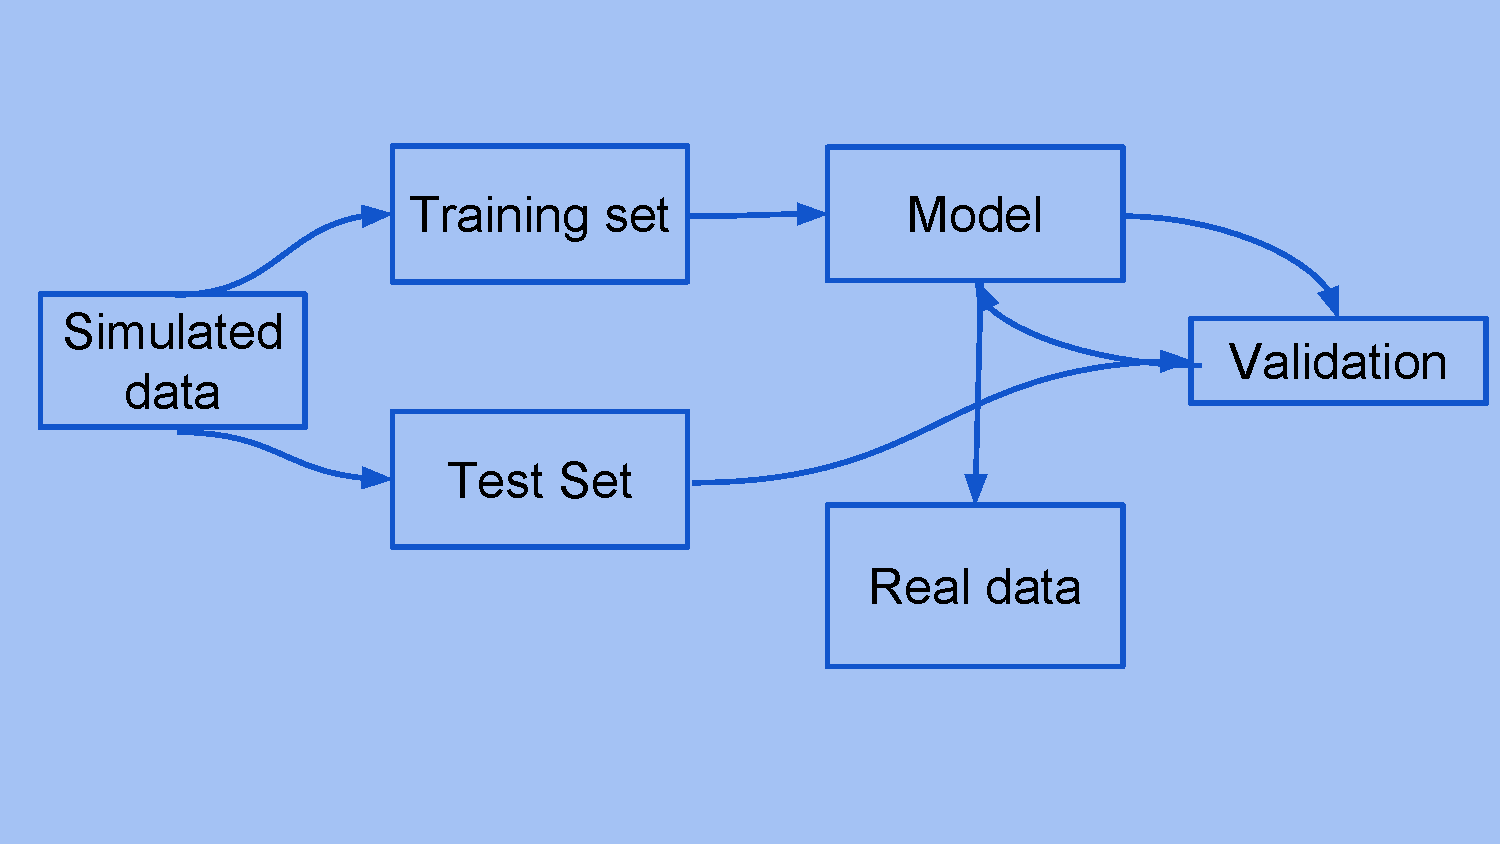
\includegraphics[scale=0.45]{./aprendizaje_supervisado.pdf}
  \end{center}
}

\frame{
 \frametitle{Simple Example:ANNz}
  ANNz: Estimating photometric redshift using artificial neural network. Collister \& Lahav 2003 (0311058)
  \begin{center}
   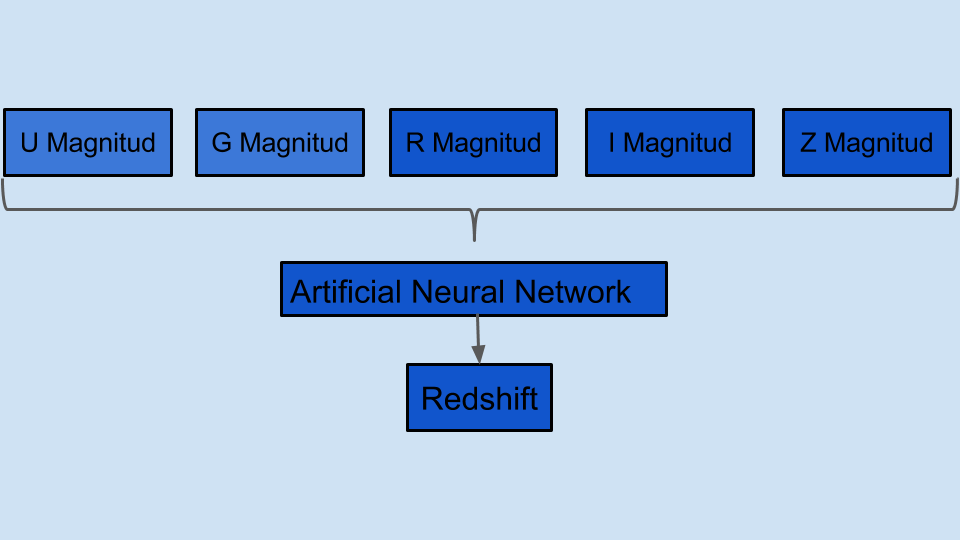
\includegraphics[scale=0.3]{./annz1.png}
  \end{center}
}
\frame{
  \begin{center}
   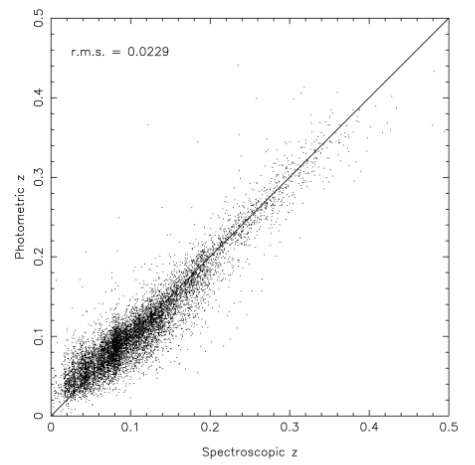
\includegraphics[scale=0.45]{./annz.png}
  \end{center}
}
%\frame{
%  \frametitle{Random Forest}
%  \begin{center}
% 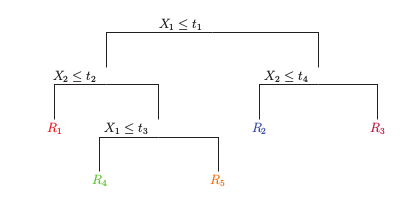
\includegraphics[scale=0.85]{./rf.png}
% % rf.png: 0x0 pixel, 300dpi, 0.00x0.00 cm, bb=
%\end{center}
%
%}

%\frame{
%  \frametitle{Support Vector Machine}
%  \begin{center}
% 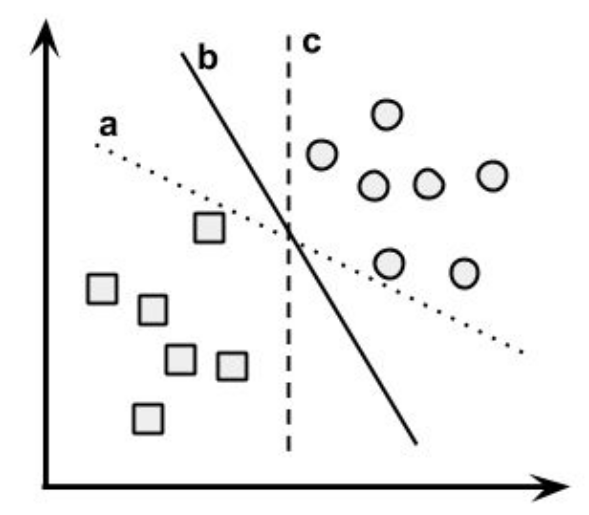
\includegraphics[scale=0.4]{./svm.png}
%
% % svm.png: 0x0 pixel, 300dpi, 0.00x0.00 cm, bb=
%\end{center}
%
%}
%\subsection{Unsupervised learning.}
%\frame{
%  \frametitle{Unsupervised Learning.}
%  \begin{center}
% 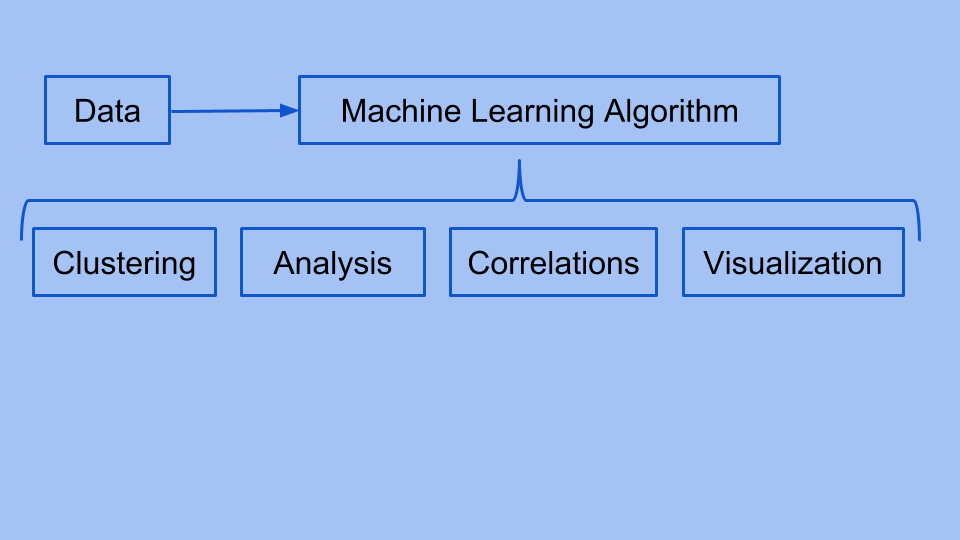
\includegraphics[scale=0.34]{./aprendizaje_nosupervisado.png}
% % aprendizaje_nosupervisado.jpg: 0x0 pixel, 300dpi, 0.00x0.00 cm, bb=
%\end{center}
%
%} 
%\frame{
% \frametitle{Mixture of Gaussians.}
% \begin{center}
% 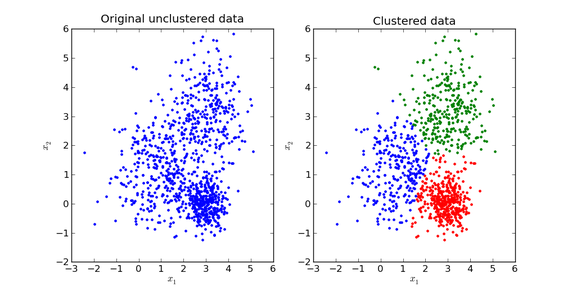
\includegraphics[scale=0.5]{./mixt_gauss.png}
% % mixt_gauss.png: 0x0 pixel, 300dpi, 0.00x0.00 cm, bb=
%\end{center}
%}
%\frame{
%\frametitle{Principal Components Analysis.}
%\begin{center}
% 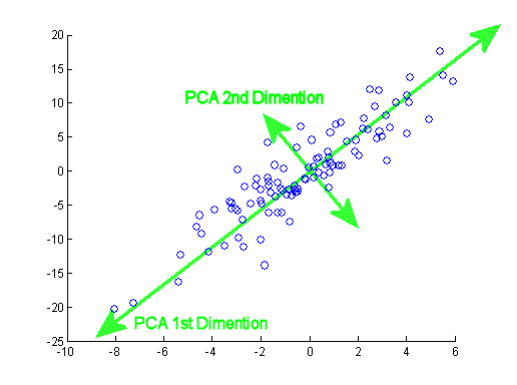
\includegraphics[scale=0.5]{./pca.png}
% % pca_example.gif: 0x0 pixel, 300dpi, 0.00x0.00 cm, bb=
%\end{center}
%
%}

\subsection{Machine Learning in physics.}
%\frame{
%  \frametitle{Machine Learning in physics.}
%  \begin{itemize}
%   \item Ann-z:
%   \item Mock Catalogues:
%   \item Galaxy Clusters mass estimation:
%   \item Morphological clasification of galaxies.
%   \item Clasification of galaxy clusters by its dynamical status.
%   \item CERN handles so much data in a single run of the LHC that 
%         it is physically impossible (I believe the figure is 50 petabytes) 
%         for human beings to manually check through the data for anomalies.
%         Instead, machine learning algorithms are used to check for anomalous
%         data and to present a summarised report for humans to work with.
%   \item Machine learning algorithms are heavily used to process satellite 
%         data in atmospheric physics as well as handle weather forecasts 
%         and predictions.
%   \item Work has begun to try and introduce machine learning tools to 
%         predict the behaviour of systems of many particles, which is of 
%         interest to condensed matter physicists, plasma physicists and chemists. 
%         This is still a developing field and might gain more momentum as 
%         time progresses.
%   \item Machine learning phases of matter(1605.01735)
%  \end{itemize}
%
%} 
%\frame{
%\begin{center}
% 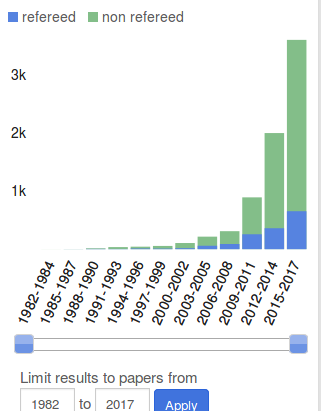
\includegraphics[scale=0.25]{./machine_learning_examples.png}
% % machine_learning_examples.png: 0x0 pixel, 300dpi, 0.00x0.00 cm, bb=
%\end{center}
%
%}
%\frame{
% \begin{figure}
% \begin{flushleft}
% 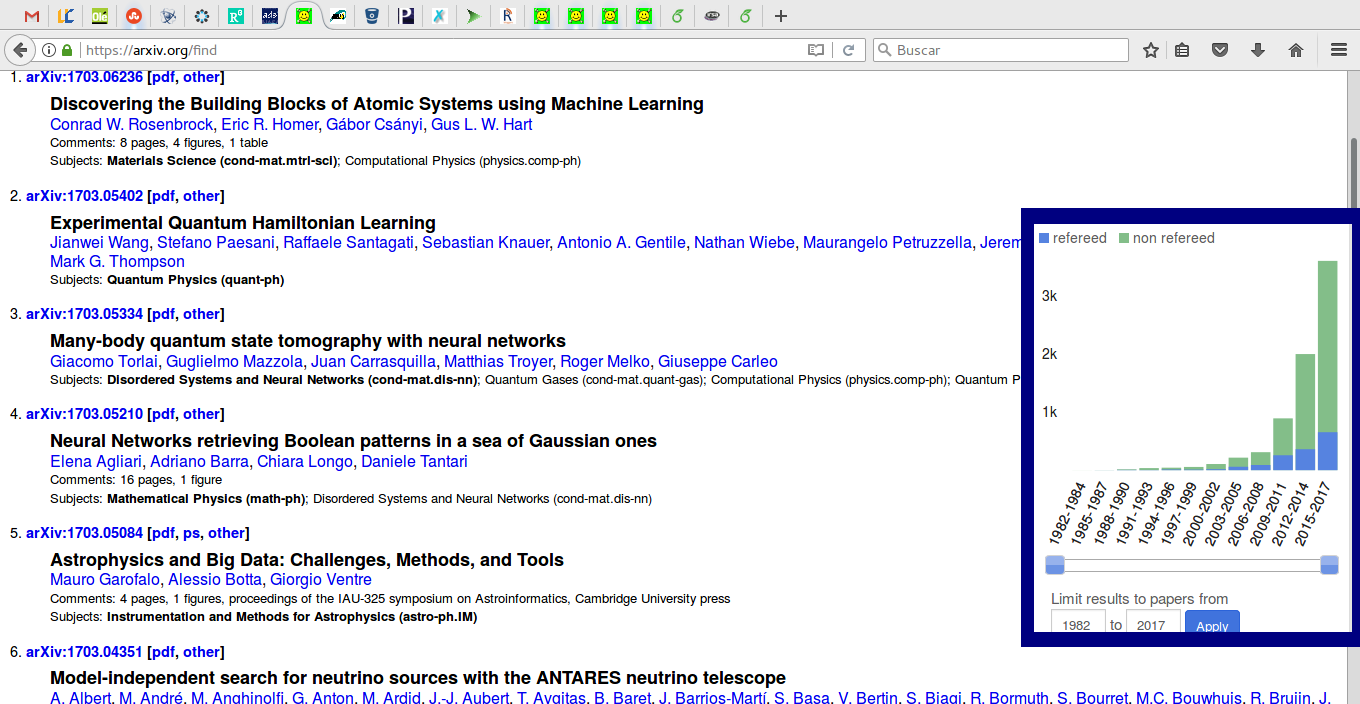
\includegraphics[scale=0.33,left]{./machine_learning_examples2.png}
%  \end{flushleft}
% \end{figure}
%}
\section{Measuring the Cosmological Parameters.}
\frame{
\tableofcontents[ 
    currentsection, 
    sectionstyle=show/hide, 
    sectionstyle=show/shaded, 
    ] 
}

%\subsection{What are the cosmological parameters?}
\frame{
  \frametitle{What are the cosmological parameters?}
  Homogeneous and isotropic Universe $\rightarrow$ FRW metric

$ds^{2}=dt^{2}-a^{2}(t)[\frac{dr^{2}}{1-kr^{2}}+r^{2}(d \theta^{2}+sin^{2} \theta d \phi^{2})] $

$(\frac{H}{H_{0}})^{2}=\Omega_{rad}a^{-4}+\Omega_{m}a^{-3}+\Omega_{\Lambda}-Kc^{2}a^{-2}$
} 
%\subsection{How can we measure the cosmological parameters?}
\frame{
  \frametitle{How can we measure the cosmological parameters?}
  \begin{center}
 %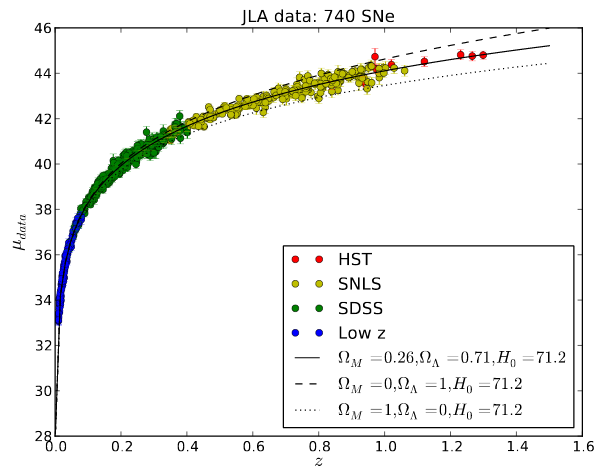
\includegraphics[scale=0.26]{./supernovas.png}
  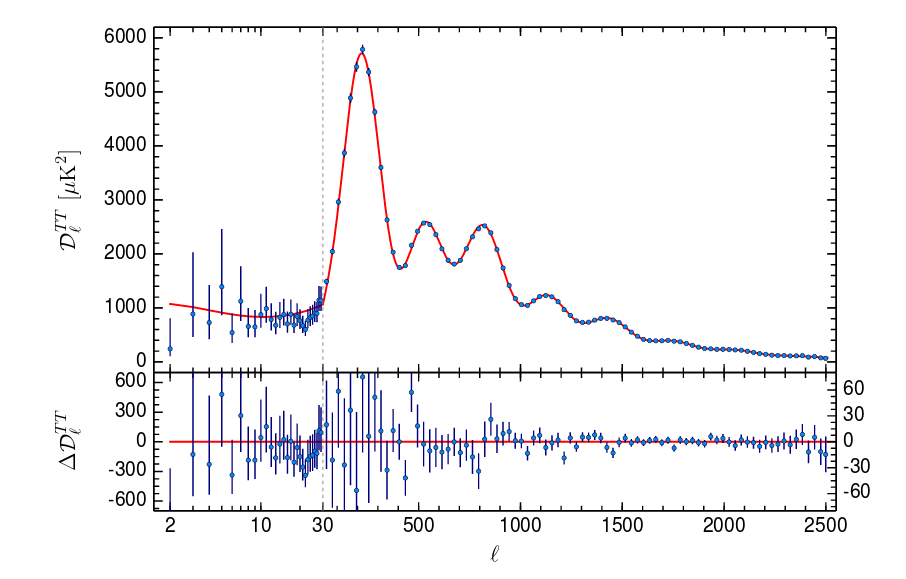
\includegraphics[scale=0.22]{./planck.png}
 % supernovas.png: 0x0 pixel, 300dpi, 0.00x0.00 cm, bb=
\end{center}
%Carvalho \& Marques 2015 (1512.07869) 
Planck Collaboration 2015 (1502.01589)
} 
%\subsection{Latest Results.}
%\frame{
%  \frametitle{Latest Results.}
%  \begin{center}
%   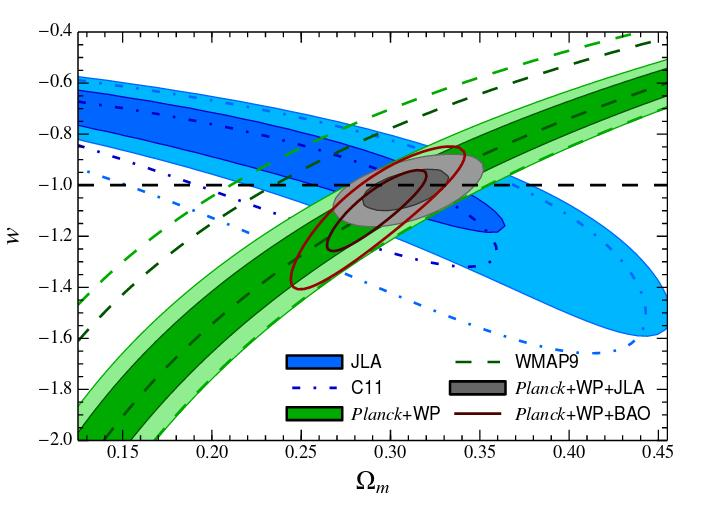
\includegraphics[scale=0.24]{./bananas.jpg}
% 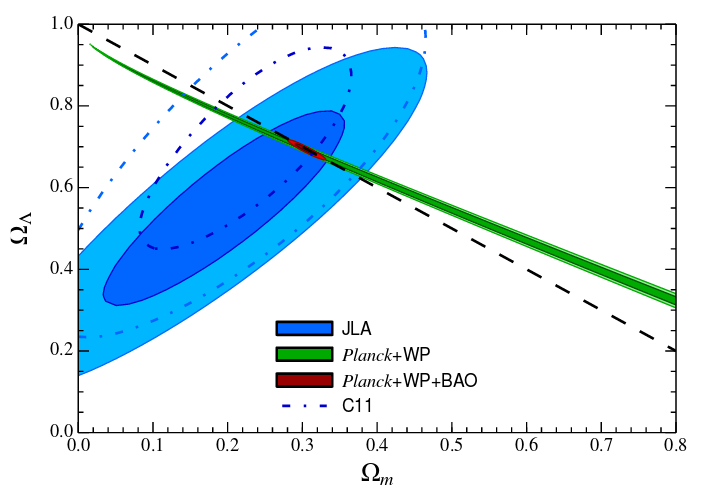
\includegraphics[scale=0.24]{./bananas2.png}
% % bananas.jpg: 0x0 pixel, 300dpi, 0.00x0.00 cm, bb=
%\end{center}
%(REFERENCIA)
%} 
%\frame{
%\begin{center}
% 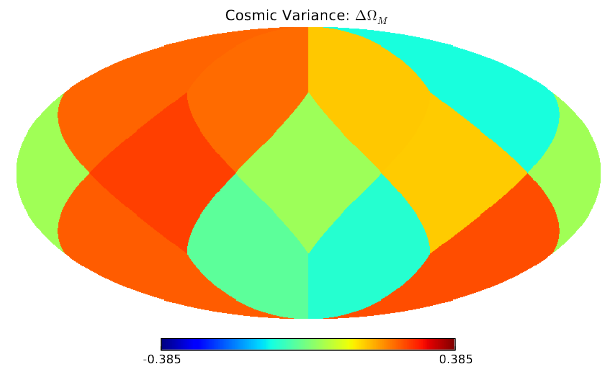
\includegraphics[scale=0.5]{./matter.png}
% % matter.png: 0x0 pixel, 300dpi, 0.00x0.00 cm, bb=
%\end{center}
%
%}
%\frame{
%\begin{center}
% 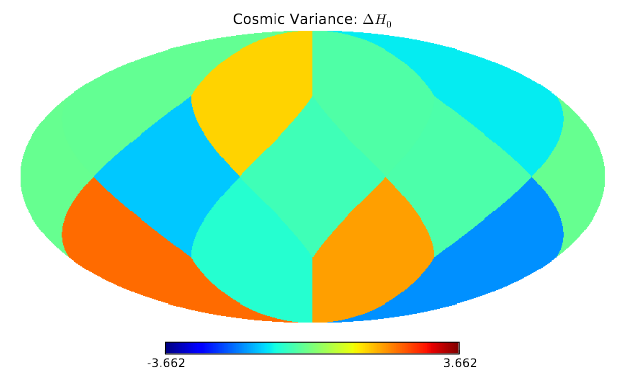
\includegraphics[scale=0.5]{./hubble.png}
 % matter.png: 0x0 pixel, 300dpi, 0.00x0.00 cm, bb=
%\end{center}
%Carvalho \& Marques (1512.07869)
%}


\subsection{The training sample.}
\frame{
\frametitle{The training sample.}
CAMB: Code for Anisotropies in the Cosmic Background 
\begin{center}
 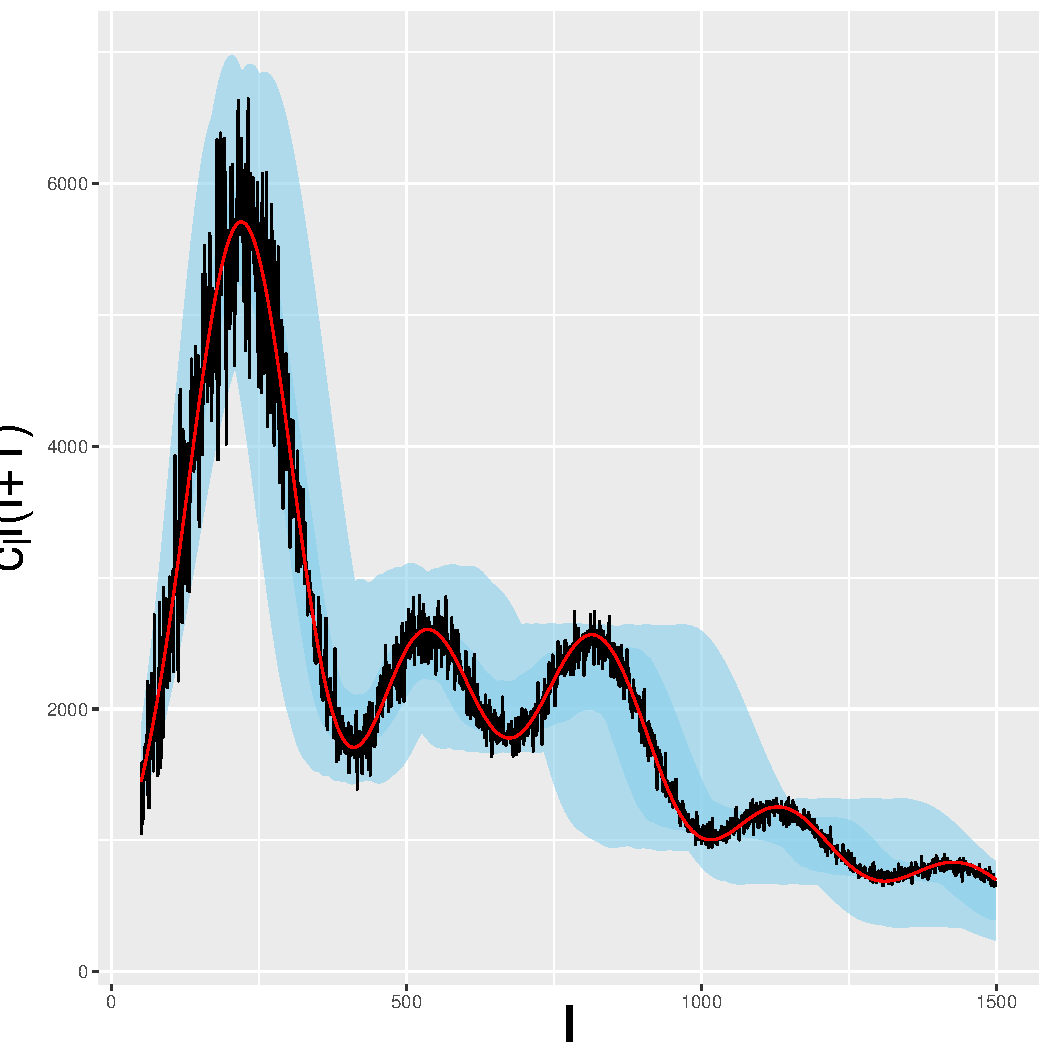
\includegraphics[scale=0.3]{./fig1_nueva.pdf}
  %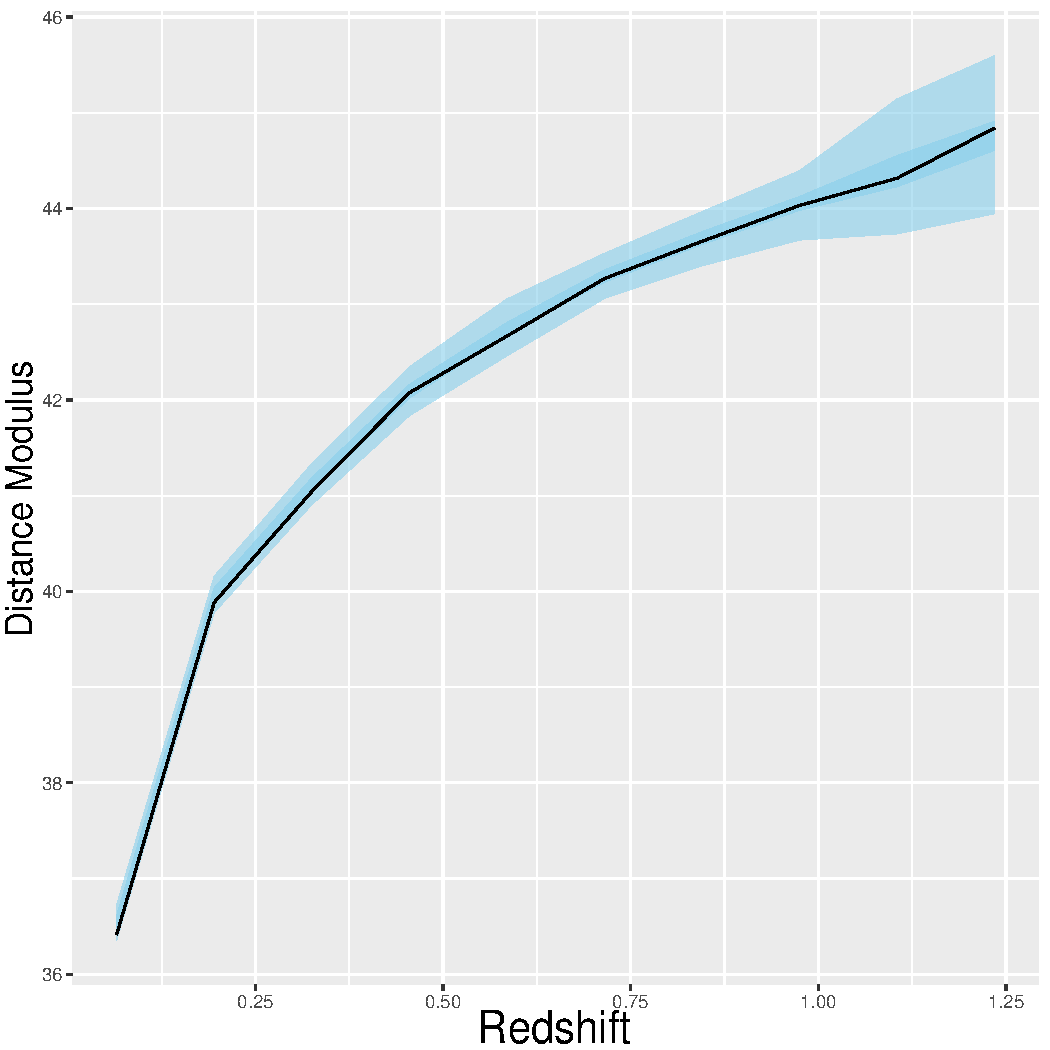
\includegraphics[scale=0.3]{./fig2_nueva.pdf}
 % fig1_nueva.pdf: 0x0 pixel, 300dpi, 0.00x0.00 cm, bb=
\end{center}

}

%\subsection{Studying different Machine Learning algorithms.}
\frame{
\begin{columns}
 \begin{column}{8cm}
\frametitle{Studying different Machine Learning algorithms.}
\begin{center}
 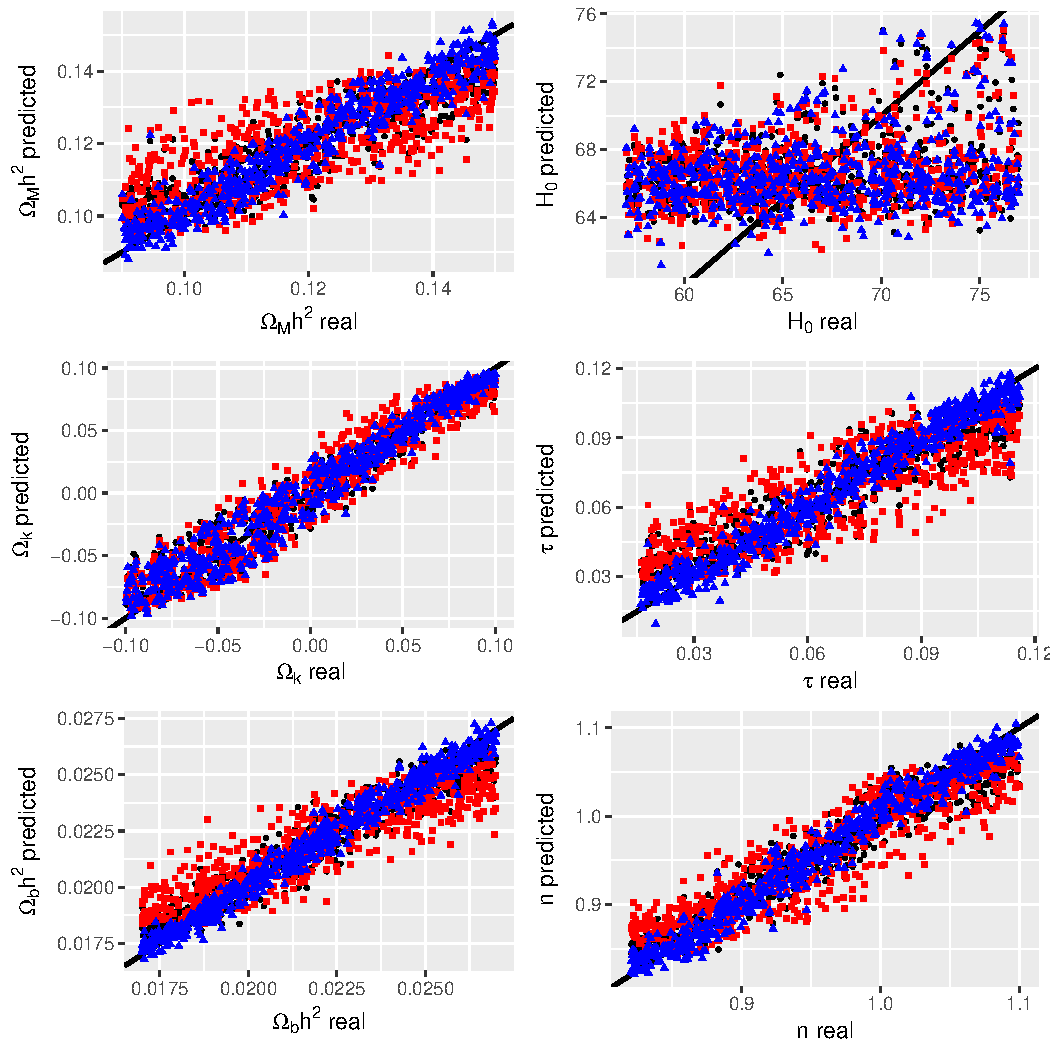
\includegraphics[scale=0.4]{./fig4_extended_30feat.pdf}
 % fig3_paper.pdf: 0x0 pixel, 300dpi, 0.00x0.00 cm, bb=
\end{center}
\end{column}
\begin{column}{4cm}
\begin{tiny}
 {\color{rojo} K-Nearest Neighbour}
 
 {Random Forest}
 
 {\color{azul} Support Vector Machine}
 
 \end{tiny}
\end{column}
\end{columns}
}

%\frame{
%Changing the minimum mutipole.

%\begin{center}
% 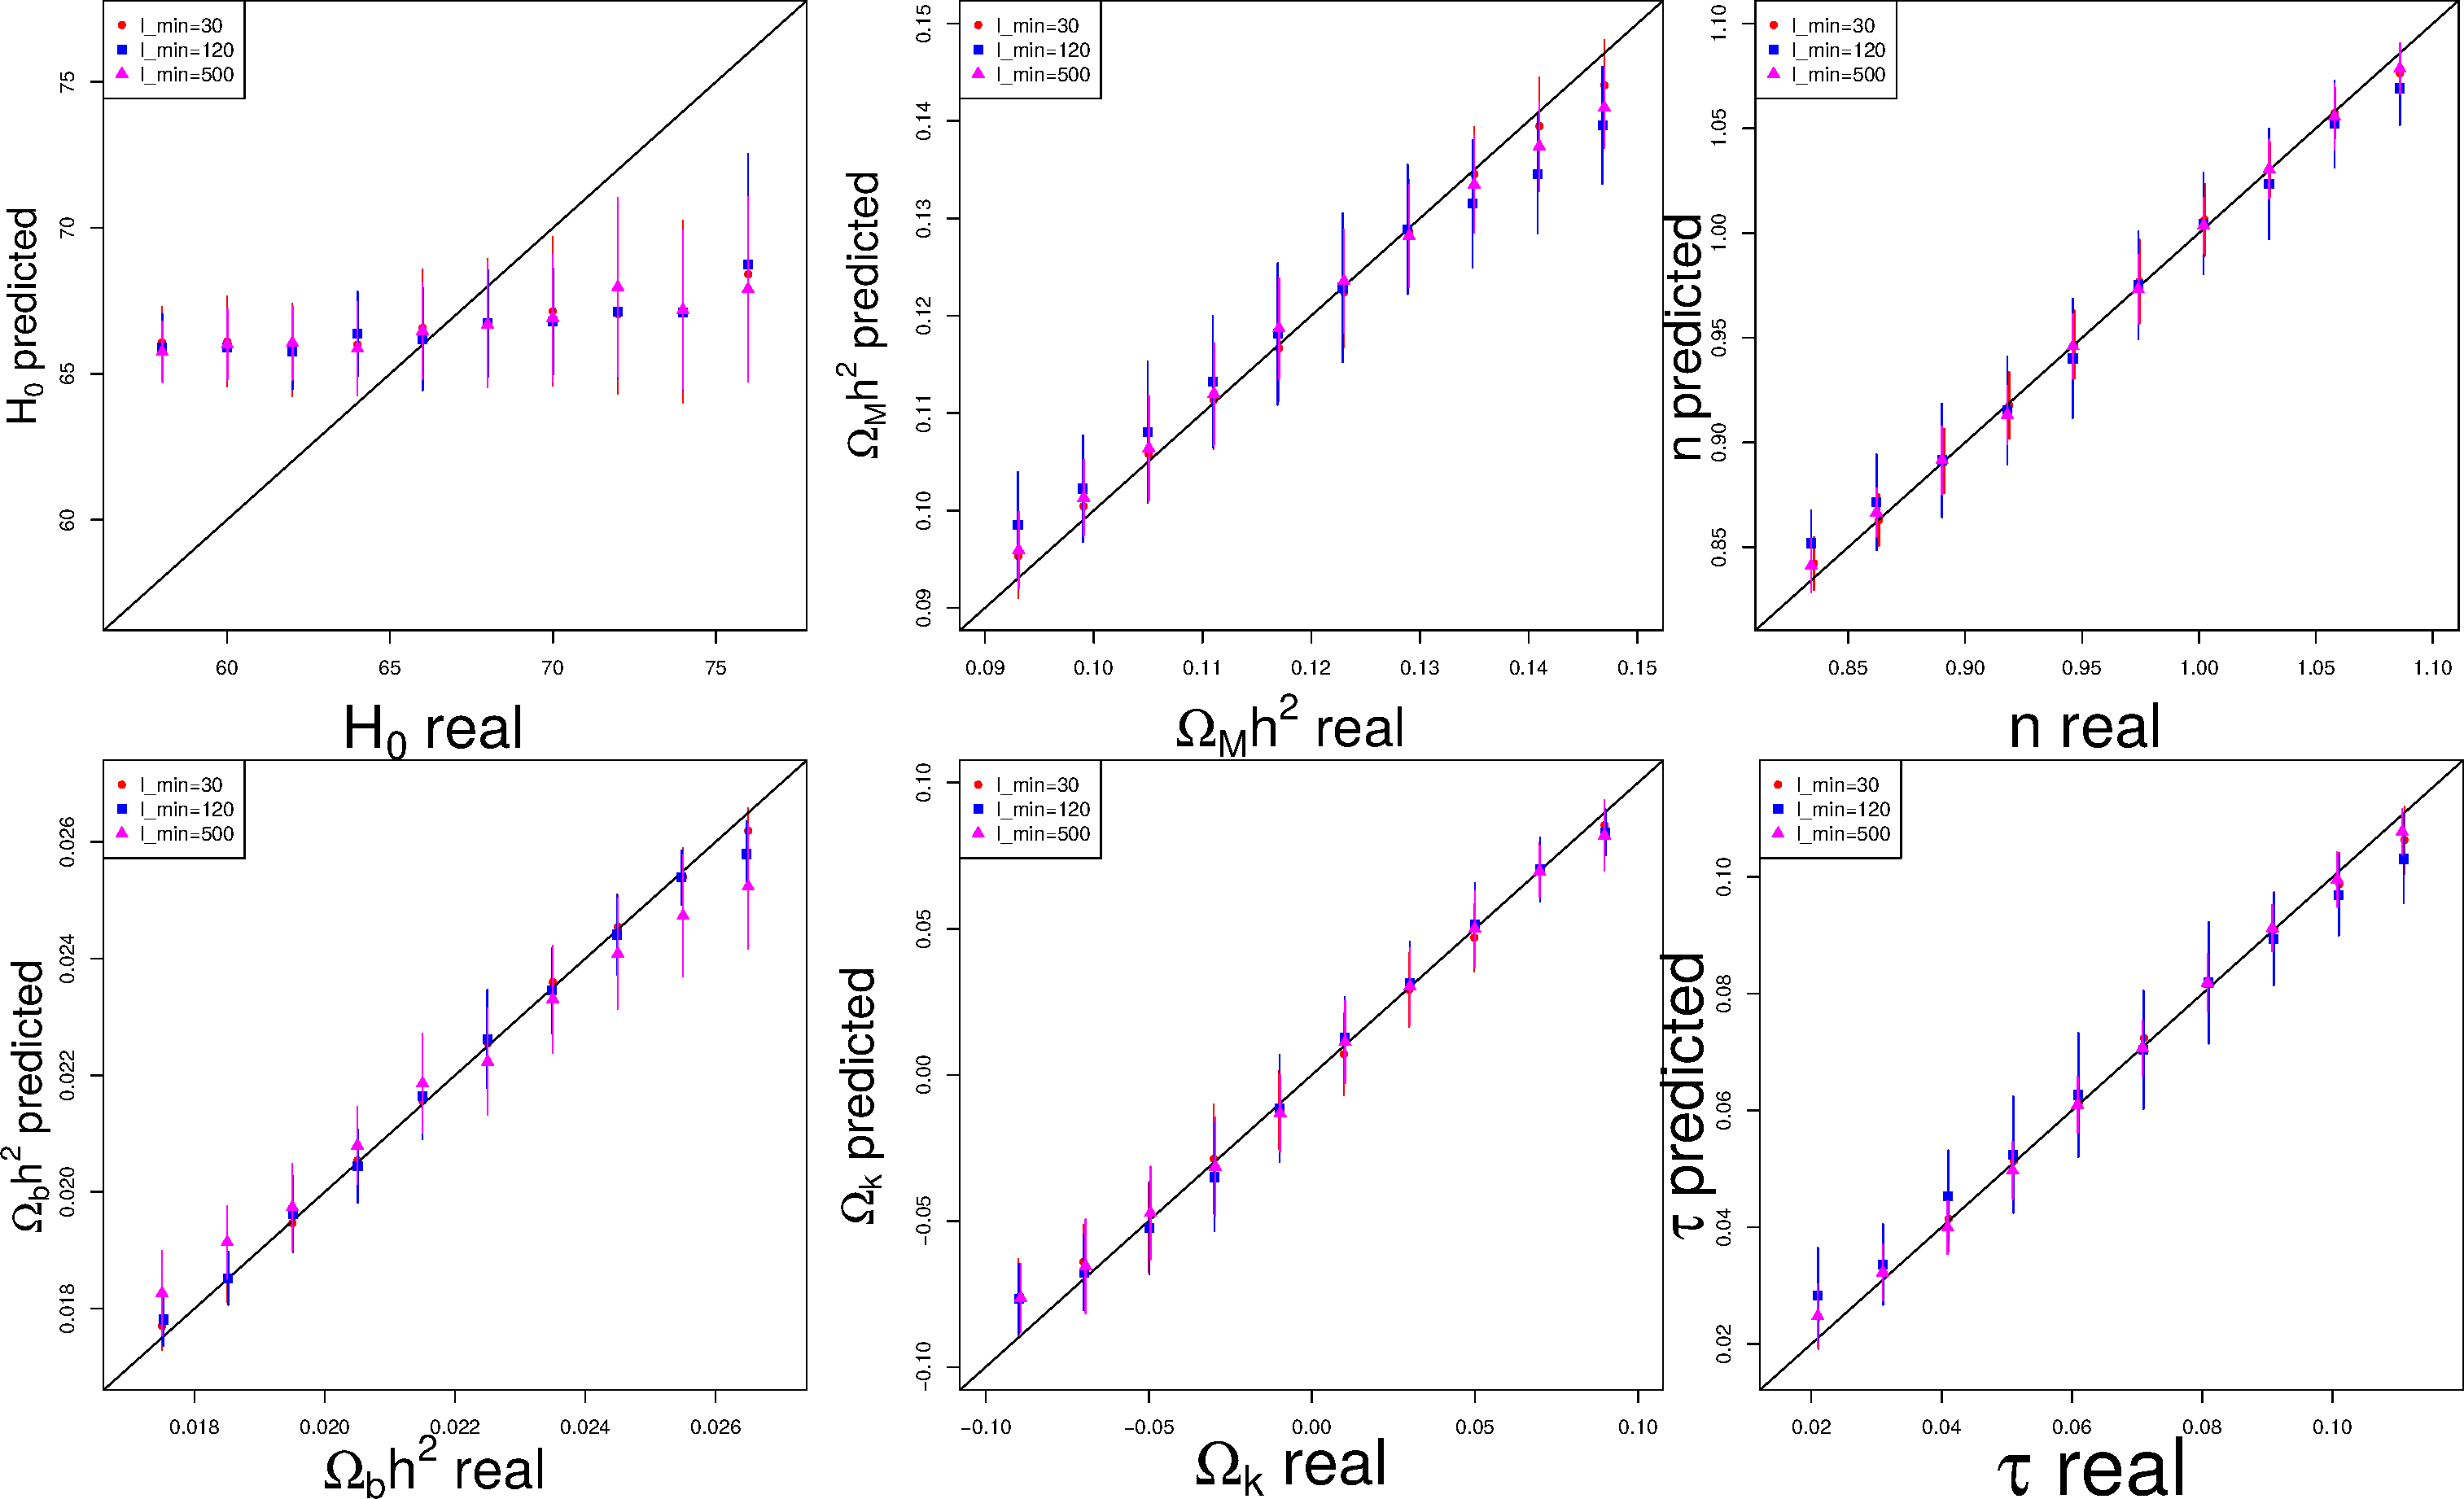
\includegraphics[scale=0.2]{./lvar.pdf}
 % lvar.pdf: 0x0 pixel, 300dpi, 0.00x0.00 cm, bb=
%\end{center}

%}
%\frame{
%\begin{center}
% 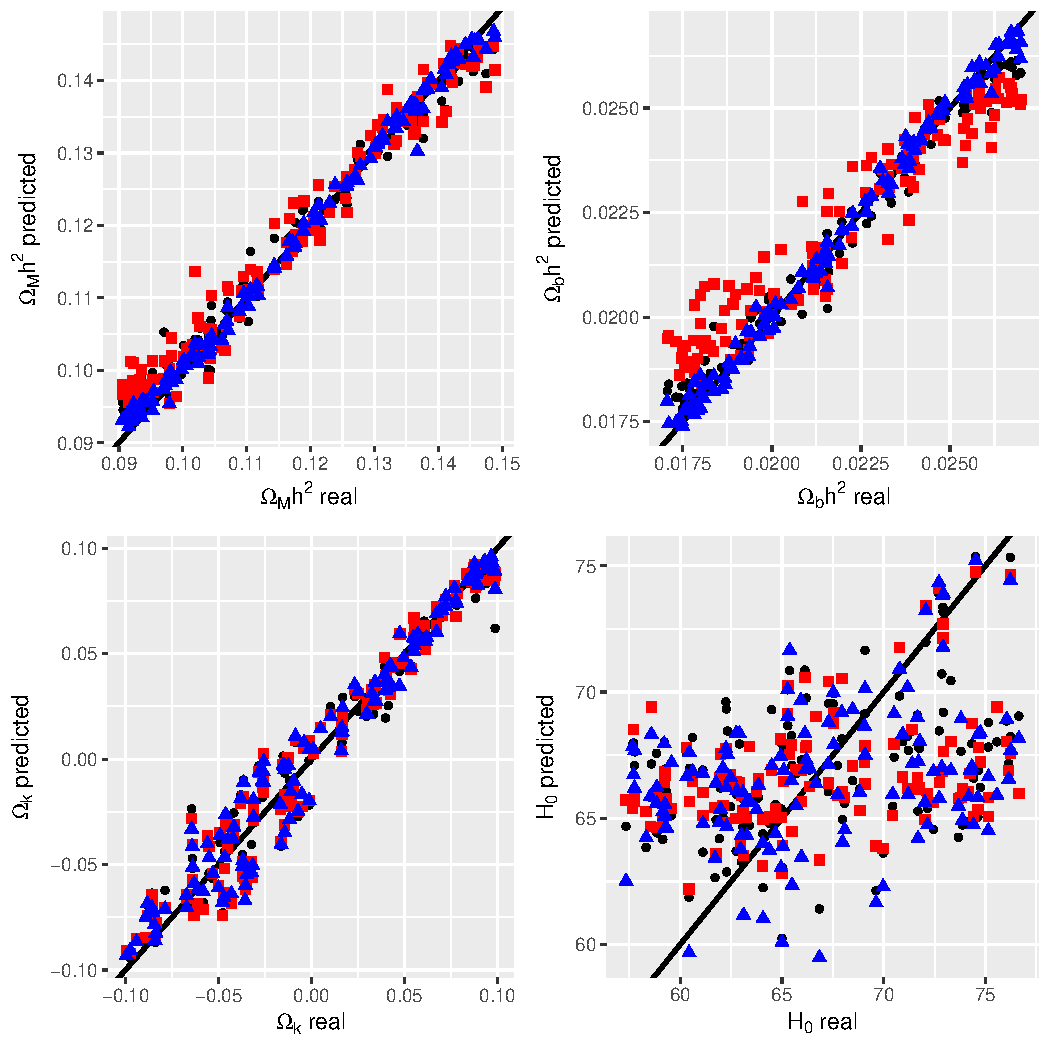
\includegraphics[scale=0.4]{./fig4_paper.pdf}
% % fig3_paper.pdf: 0x0 pixel, 300dpi, 0.00x0.00 cm, bb=
%\end{center}
%}
%\frame{
%\begin{center}
% 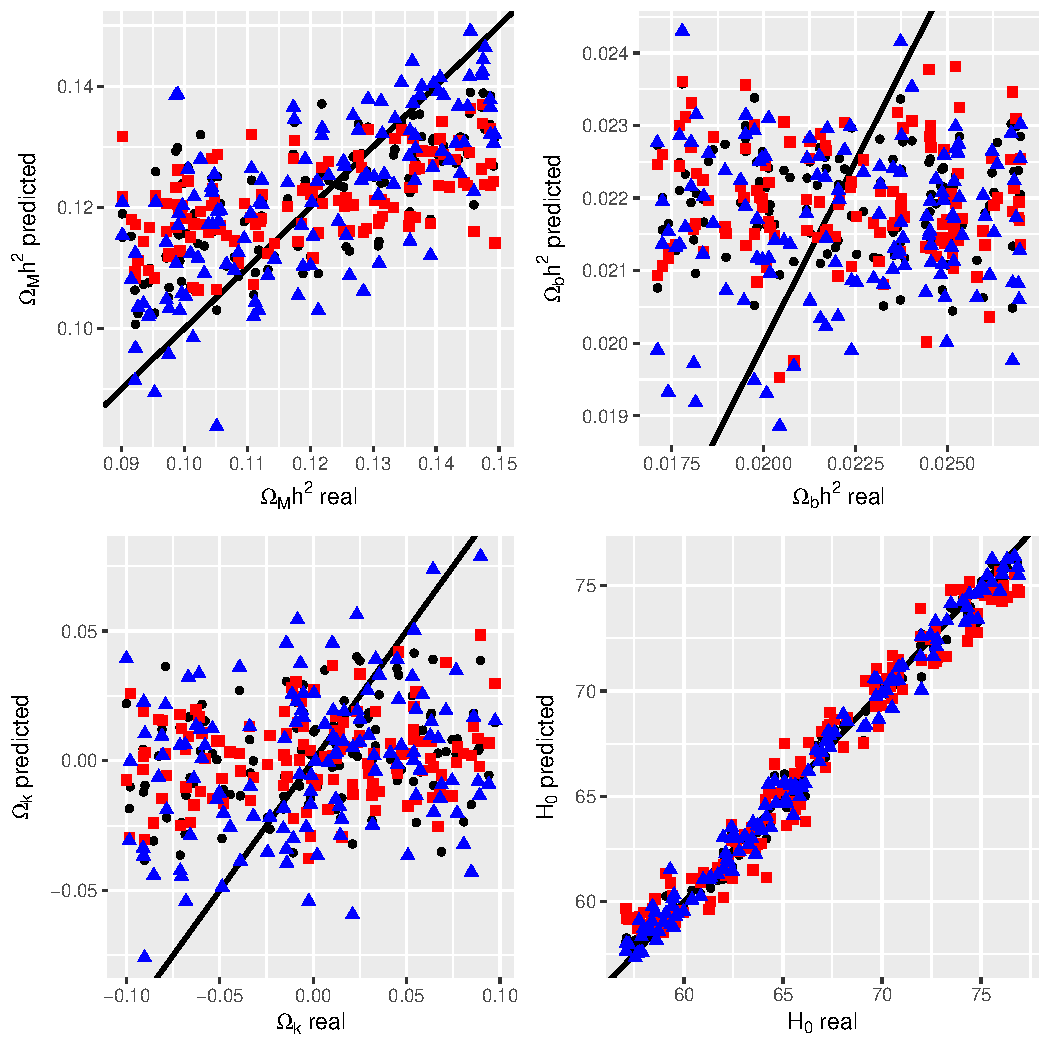
\includegraphics[scale=0.4]{./fig5_paper.pdf}
% % fig3_paper.pdf: 0x0 pixel, 300dpi, 0.00x0.00 cm, bb=
%\end{center}
%}
\subsection{Applications.}
\frame{
\frametitle{Measuring the cosmological parameters angular distributions. }

\begin{center}
 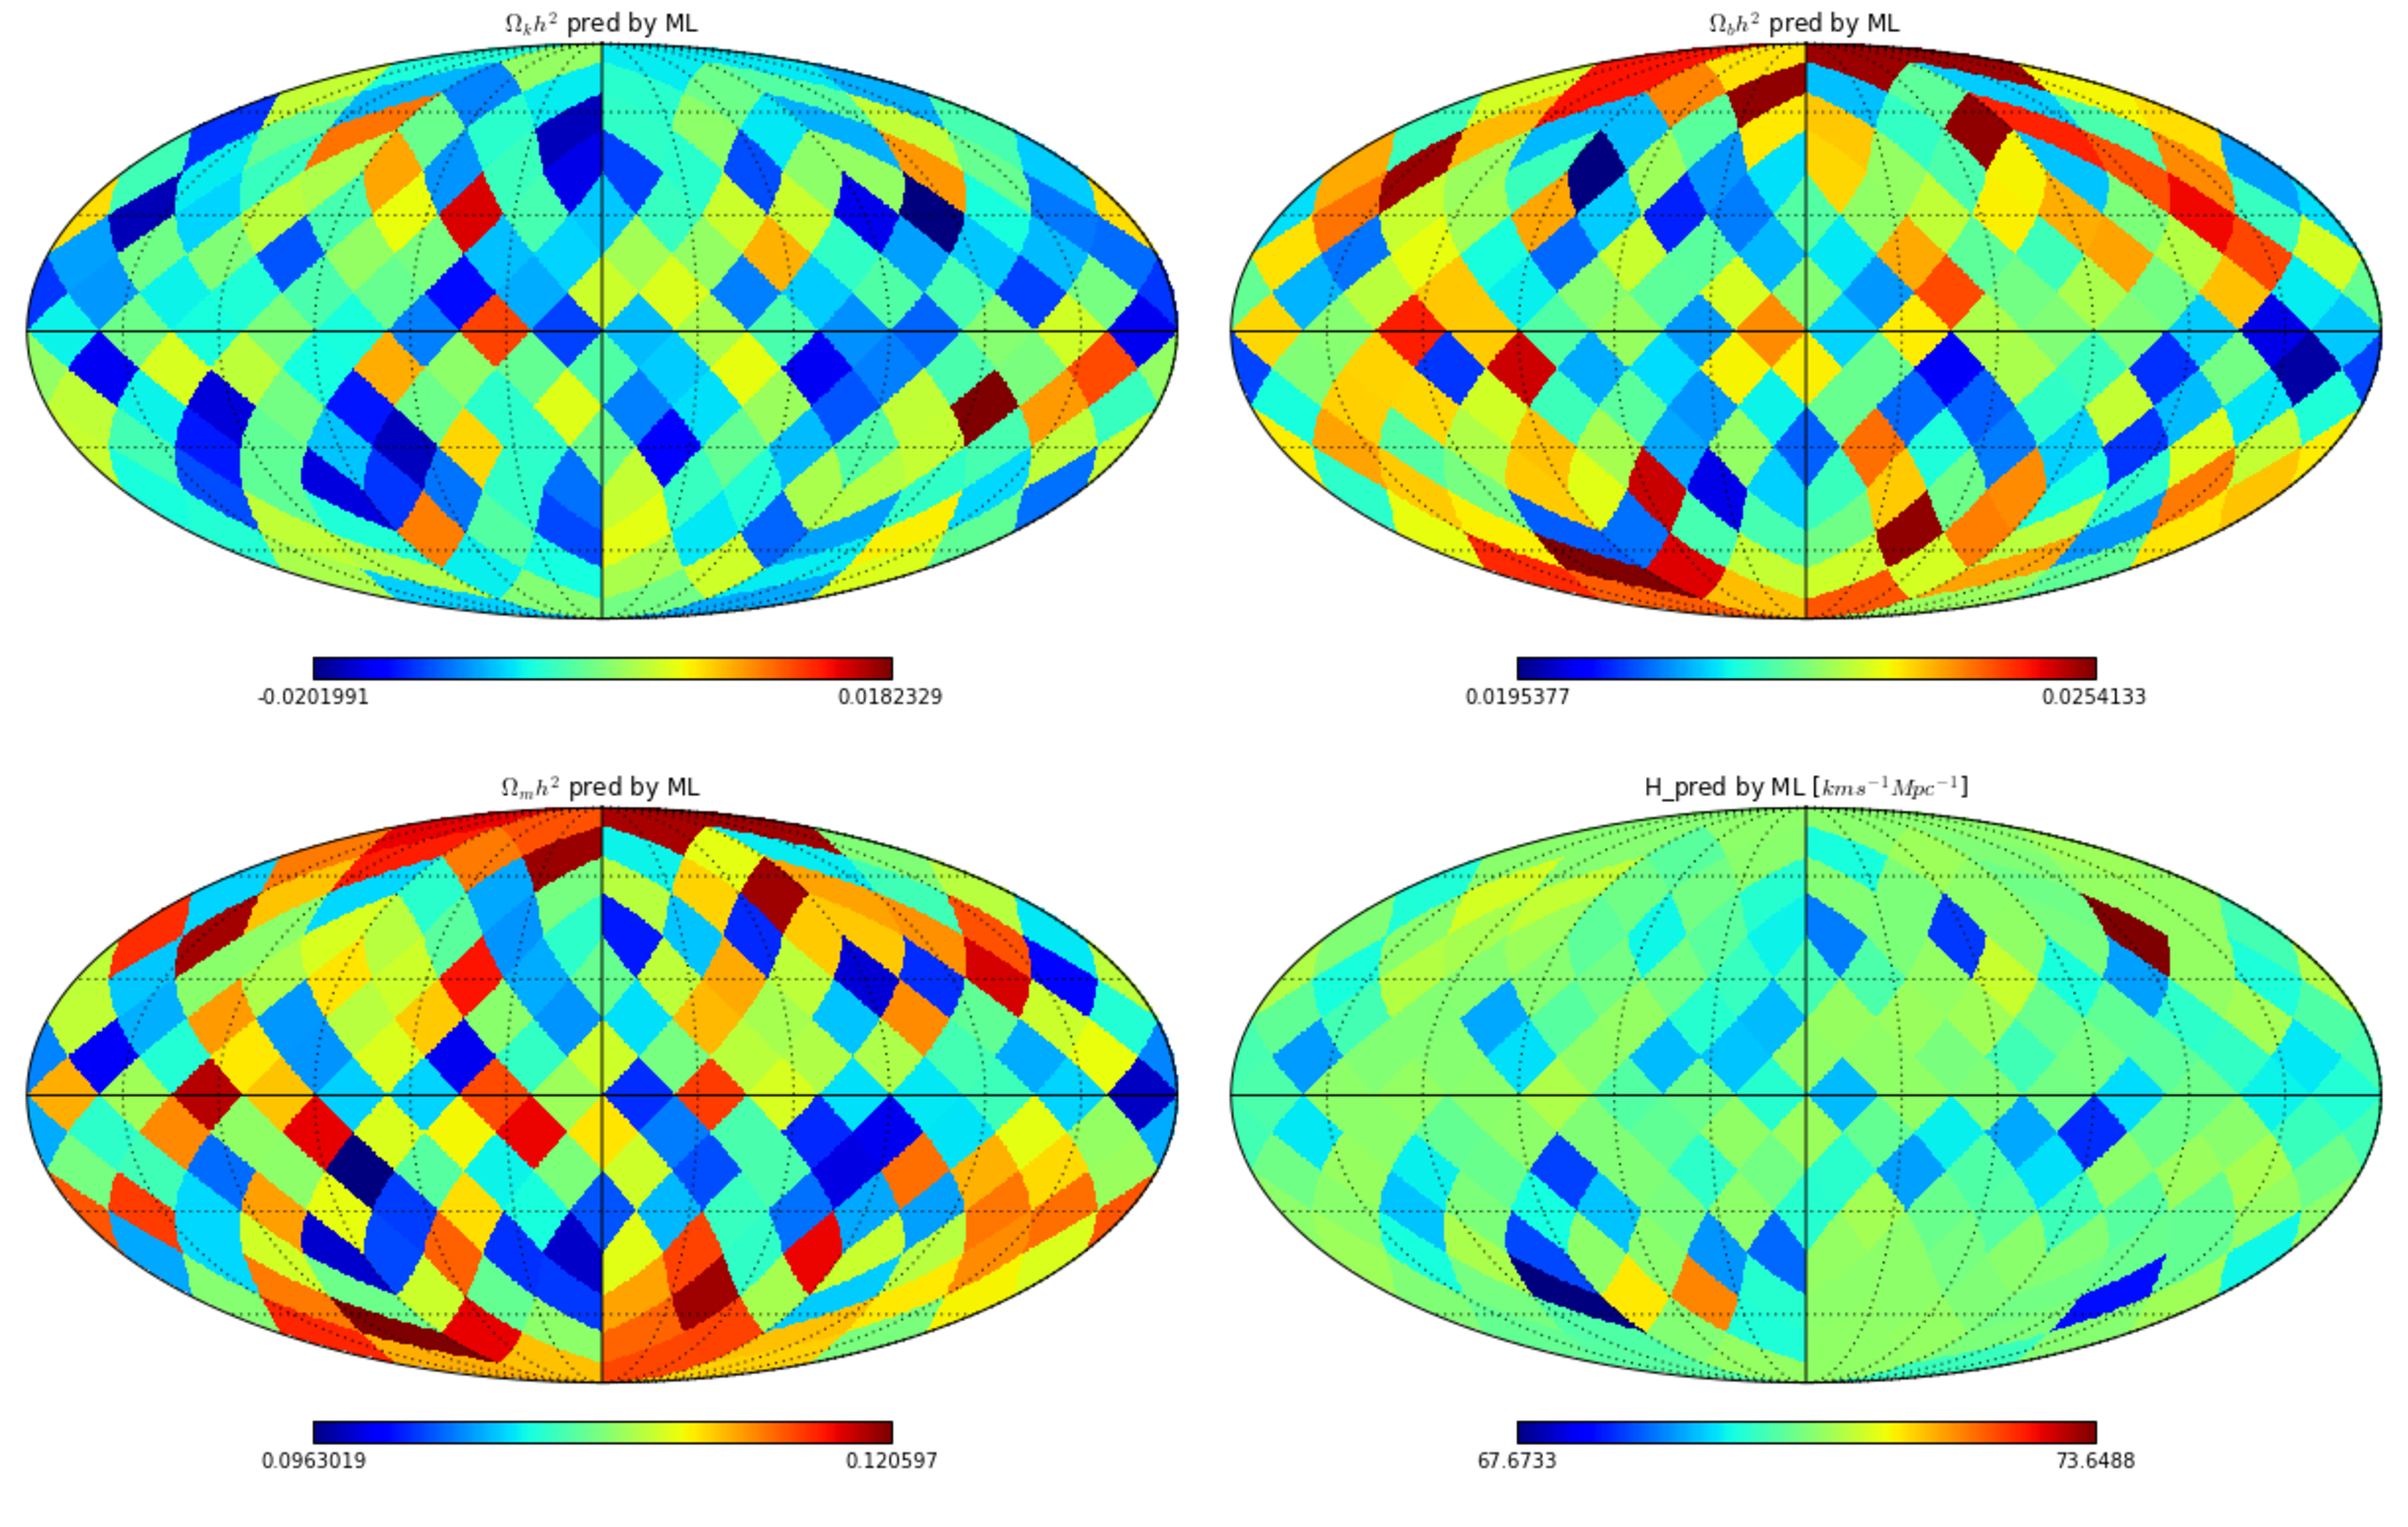
\includegraphics[scale=0.22]{./fig7_paper.pdf}
 % fig7_paper.pdf: 0x0 pixel, 300dpi, 0.00x0.00 cm, bb=
\end{center}
de los Rios \& Dominguez et al. (in preparation)
}

\frame{
\begin{center}
\hspace{-2.1cm}
 
\includegraphics[scale=0.5]{./Stranger_Things_logo.png}
 % Stranger_Things_logo.png: 0x0 pixel, 300dpi, 0.00x0.00 cm, bb=
\end{center}

}

\frame{
 \begin{center}
 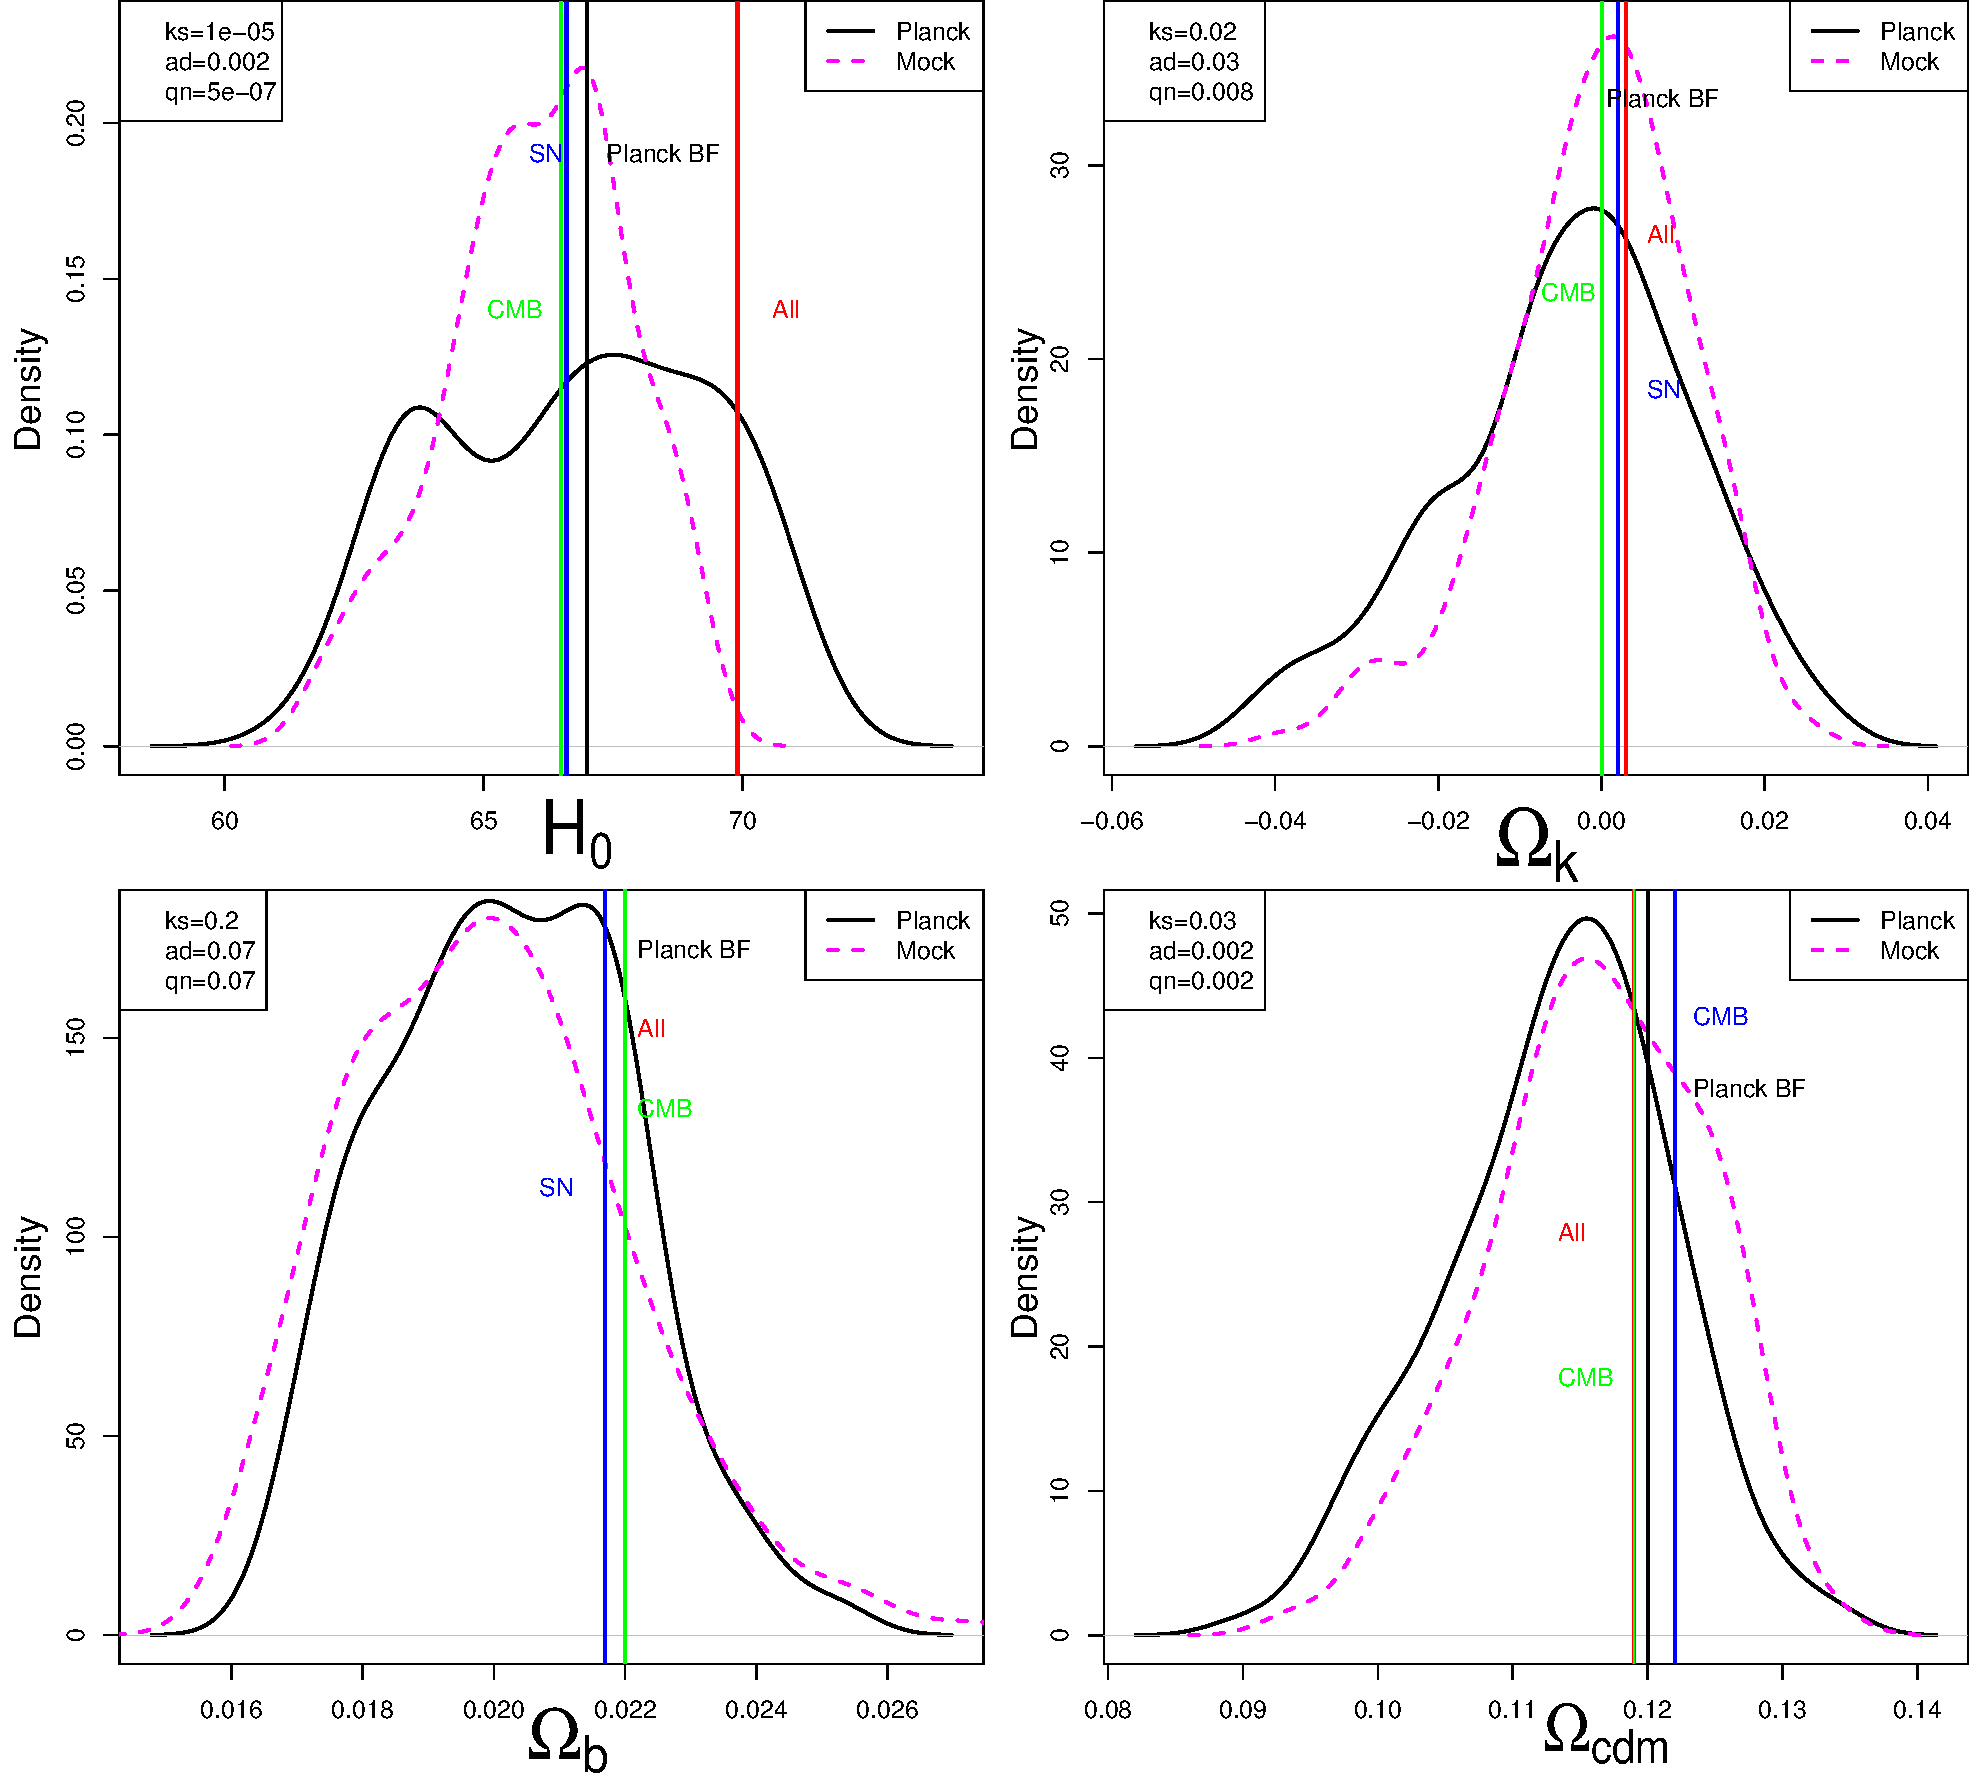
\includegraphics[scale=0.18]{./comparaciones.pdf}
 % comparaciones.pdf: 0x0 pixel, 300dpi, 0.00x0.00 cm, bb=
\end{center}

}


\frame{
\frametitle{Hemispheric Asymmetry. de los Rios \& Dominguez (in preparation).}
\begin{figure}[t!]
 \centering
 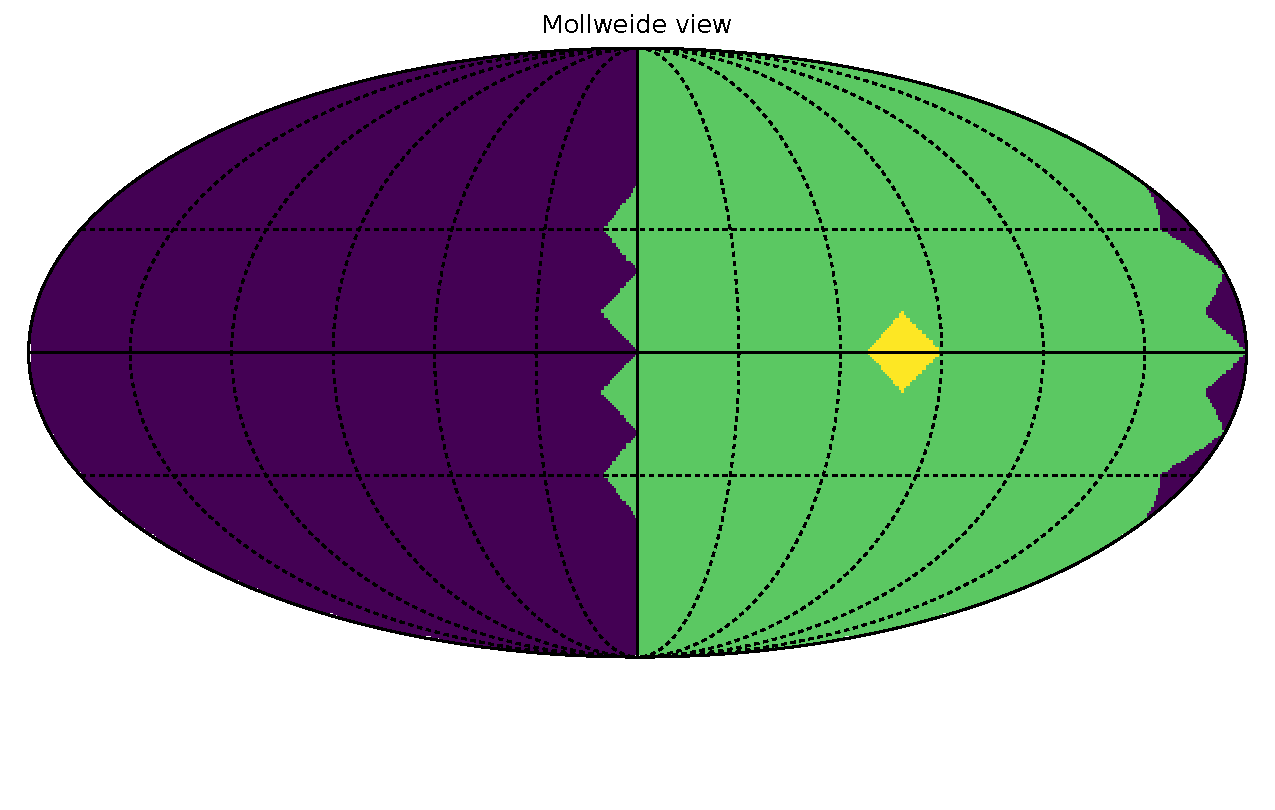
\includegraphics[scale=0.5]{./example_pi_2.pdf}
 % example_pi_2.pdf: 0x0 pixel, 300dpi, 0.00x0.00 cm, bb=
\end{figure}
}

\frame{
\begin{figure}[t!]
 \centering
 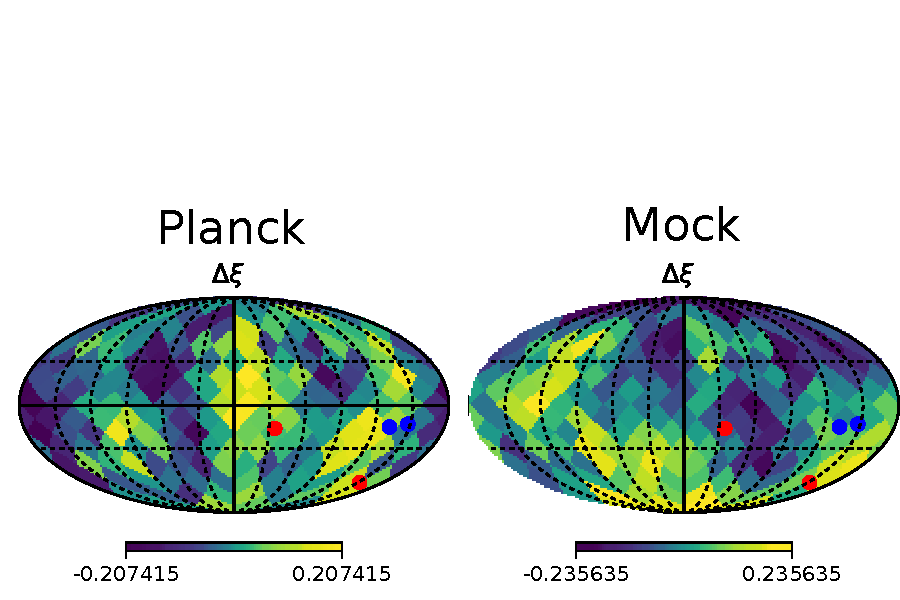
\includegraphics[scale=0.65]{./hemispheric_d2diff_pi_2.pdf}
 % hemispheric_d2diff_pi_2.pdf: 0x0 pixel, 300dpi, 0.00x0.00 cm, bb=
\end{figure}
\begin{small}
 
$\xi^{2}=(\frac{H_{pl}-H}{\sigma_{H}})^{2}+(\frac{\Omega_{m,pl}-\Omega_{m}}{\sigma_{\Omega_{m}}})^{2}+(\frac{\Omega_{b,pl}-\Omega_{b}}{\sigma_{\Omega_{b}}})^{2}+
(\frac{\Omega_{k,pl}-\Omega_{k}}{\sigma_{\Omega_{k}}})^{2}+(\frac{\tau_{pl}-\tau}{\sigma_{\tau}})^{2}+(\frac{n_{pl}-n}{\sigma_{n}})^{2}$

\end{small}
}
\section{Final Remarks.}
\frame{
\tableofcontents[ 
    currentsection, 
    sectionstyle=show/hide, 
    sectionstyle=show/shaded, 
    ] 
}
\frame{
\frametitle{Final Remarks}
\begin{small}
 

\begin{itemize}
 \item We developed a machine learning technique that estimate the cosmological parameters in a more efficient way withouth losing precision.
 \item This technique can be easily extended to use more cosmological information as features (BAO, correlation function, SZ emission, etc.).
 %\item We do not found statistically significant departures from what is expected in an homogeneous and isotropic universe, with the possible
 %exception of a bi-modal $H_{0}$ distribution.
 \item As a first application we study the angular distribution of the cosmological parameters and the Hemispherical Asymmetry.
 \item We do not found any significant departure from what is expected in an homogeneous and isotropic univese, but 
       we found some features in the distributions that may come from the pixelization.
 \item We will extend the parameters space and add polarization information in a forthcoming work.
 \item We will analyze the correlations between the angular distribution of the cosmological parameters and the large scale structure (voids, filaments, etc.) 
\end{itemize}
\end{small}

}
\frame{
 \begin{center}
 
\includegraphics[scale=0.45]{./thankyou.png}
 % comparaciones.pdf: 0x0 pixel, 300dpi, 0.00x0.00 cm, bb=
\end{center}

}

\end{document}

